\documentclass{standalone}

\usepackage{tikz}
\usepackage{circuitikz}

\tikzset{block/.style = {draw, fill=white, very thick, rectangle, minimum height=1cm, minimum width=2cm},
         lblock/.style={draw,fill=white,very thick, rectangle, minimum height=3cm, minimum width=1cm},
         sum/.style= {draw, fill=white, very thick, circle, node distance=0.5cm}}

         
\begin{document}
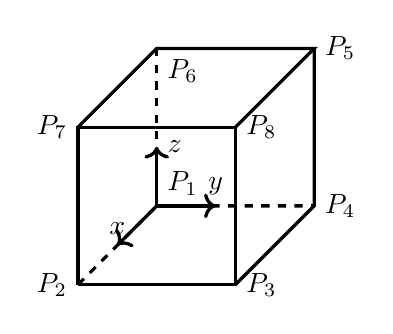
\begin{tikzpicture}[scale=2]
    \draw[-,very thick](0,0)node[left]{$P_2$}--(1,0)node[right]{$P_3$}--(1,1)node[right]{$P_8$}--(0,1)node[left]{$P_7$}--(0,0);
    \draw[dashed,very thick](0,0)--(0.5,0.5)node[above right]{$P_1$}--(1.5,0.5)node[right]{$P_4$};
    \draw[dashed,very thick](0.5,0.5)--(0.5,1.5)node[below right]{$P_6$};
    \draw[-,very thick](1,1)--(1.5,1.5)node[right]{$P_5$}--(0.5,1.5)--(0,1);
    \draw[-,very thick](1,0)--(1.5,0.5)--(1.5,1.5);
    \draw[->,very thick](0.5,0.5)--(0.25,0.25)node[above]{$x$};
    \draw[->,very thick](0.5,0.5)--(0.875,0.5)node[above]{$y$};
    \draw[->,very thick](0.5,0.5)--(0.5,0.875)node[right]{$z$};
\end{tikzpicture}
\end{document}